\section{Putting it together}
\label{sec:decoding}

With the pieces of the previous sections, the decoder and encoder number two fit in a page each
(Algorithms~\ref{alg:decode} and~\ref{alg:encode}). Both work on a single $X\times Y$ array of
reals in which every subband occupies the rectangle that Algorithm~\ref{alg:tree} assigns to
it, so the wavelet transform runs in place, as in Figure~\ref{fig:a002subbands}.

\begin{algorithm}[ht]
  \caption{The WSQ decoder.}
  \label{alg:decode}
  \begin{algorithmic}[1]
    \Require a WSQ file
    \Ensure an $X \times Y$ image with 8-bit samples
    \State read the file (Algorithm~\ref{alg:parse}): $X$, $Y$, $M$, $R$; filters; $C$, $Q_k$, $Z_k$; Huffman tables; blocks
    \State $(\mathcal{S}, \mathcal{L}) \gets \Call{BuildTree}{X, Y}$ \Comment{Algorithm~\ref{alg:tree}}
    \State $N \gets \sum_{k:\,Q_k > 0} X_kY_k$ \Comment{number of indices to decode}
    \State $p \gets$ empty list
    \For{each block, in order}
      \State append the indices of the block to $p$, using table $T_d$ and expecting $N - |p|$ more \Comment{Algorithm~\ref{alg:huffdecode}}
    \EndFor
    \State \textbf{fail} unless $|p| = N$
    \State $A \gets$ zero array of $Y$ rows and $X$ columns
    \For{$k \gets 0$ \textbf{to} $63$ with $Q_k > 0$}
      \State take the next $X_kY_k$ values of $p$, row by row, as $p_k(m,n)$
      \State $A$ at the rectangle of subband $k$ $\gets \hat a_k(m,n)$ by Eq.~\eqref{eq:dequantize}
    \EndFor
    \State \Call{Inverse}{$A$} \Comment{Algorithm~\ref{alg:transform2d}}
    \State $\hat I(m,n) \gets \min(255, \max(0, \floor{A(m,n)\,R + M + \frac12}))$ \Comment{Eq.~\eqref{eq:denormalize}}
  \end{algorithmic}
\end{algorithm}

\begin{algorithm}[ht]
  \caption{Encoder number two.}
  \label{alg:encode}
  \begin{algorithmic}[1]
    \Require an $X \times Y$ image $I$ with 8-bit samples; target rate $r$ in bits per pixel
    \Ensure a WSQ file
    \State $M, R \gets$ Eq.~\eqref{eq:MR};\ $A(m,n) \gets (I(m,n) - M)/R$
    \State $(\mathcal{S}, \mathcal{L}) \gets \Call{BuildTree}{X, Y}$;\ \Call{Forward}{$A$} \Comment{Algorithms~\ref{alg:tree}, \ref{alg:transform2d}}
    \State $\sigma_k^2 \gets$ window variances for $k = 0..3$ (Eqs.~\eqref{eq:window}, \eqref{eq:variance})
    \State \textbf{if} $\sum_{k=0}^{3}\sigma_k^2 > 20\,000$ \textbf{then} window variances for $k = 4..59$
           \textbf{else} full-subband variances for $k = 0..59$
    \State $Q_k, Z_k \gets$ Algorithm~\ref{alg:binwidths};\ $C \gets 0.44$
    \For{$k \gets 0$ \textbf{to} $59$ with $Q_k > 0$}
      \State $p_k(m,n) \gets$ Eq.~\eqref{eq:quantize} on the coefficients of subband $k$
    \EndFor
    \State symbols of blocks 1, 2, 3 (subbands 0--18, 19--51, 52--59) $\gets$ Algorithm~\ref{alg:tokenize}
    \State table 0 from the counts of block 1, table 1 from the counts of blocks 2 and 3 \Comment{Algorithm~\ref{alg:hufftable}}
    \State write \marker{SOI}; optionally a \marker{COM} with \texttt{NIST\_COM}; \marker{DTT}; \marker{DQT}; \marker{SOF}
    \For{$b \gets 1$ \textbf{to} $3$}
      \State write \marker{DHT} for the block's table if not yet written; write \marker{SOB}
      \State write the codes and extra bits of the block's symbols, MSB first; pad with 1-bits; stuff \hex{00} after each \hex{FF}
    \EndFor
    \State write \marker{EOI}
  \end{algorithmic}
\end{algorithm}

\subsection{What the decoder sees}

Figure~\ref{fig:rates} shows a detail of image \texttt{a002} after compression at three target
rates with the NIST encoder, and Table~\ref{tab:rates} gives the numbers for the whole image.
The usual rate for 500 ppi images is 0.75 bits per pixel; 0.25 is far below anything used in
practice and is included to make the effect of coarse quantization visible.

\begin{figure}[ht]
  \centering
  % Generated by tools/gen_figures.py; do not edit by hand.
\begin{tabular}{@{}c@{\hspace{2mm}}c@{\hspace{2mm}}c@{\hspace{2mm}}c@{}}
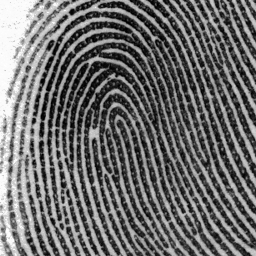
\includegraphics[width=0.24\linewidth]{images/a002-detail-original} & 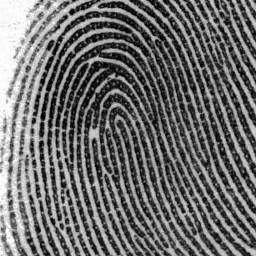
\includegraphics[width=0.24\linewidth]{images/a002-detail-225} & 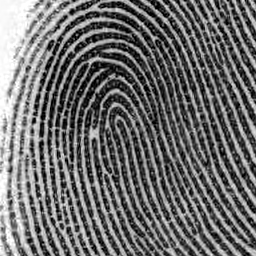
\includegraphics[width=0.24\linewidth]{images/a002-detail-075} & 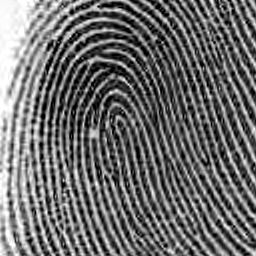
\includegraphics[width=0.24\linewidth]{images/a002-detail-025}\\
original & $r = 2.25$ & $r = 0.75$ & $r = 0.25$\\
\end{tabular}

  \caption{A $256 \times 256$ detail of \texttt{a002}: original and decoded after compression
  with the NIST encoder at three target rates.}
  \label{fig:rates}
\end{figure}

% Generated by tools/gen_figures.py; do not edit by hand.
\begin{table}[ht]
  \centering\small
  \begin{tabular}{@{}rrrrr@{}}
    \toprule
    target $r$ & file size (bytes) & compression ratio & bits per pixel & PSNR (dB)\\
    \midrule
    2.25 & 339\,730 & 4.3\,:\,1 & 1.86 & 34.01\\
    0.75 & 87\,700 & 16.7\,:\,1 & 0.48 & 26.97\\
    0.25 & 28\,784 & 50.7\,:\,1 & 0.16 & 23.29\\
    \bottomrule
  \end{tabular}
  \caption{Image \texttt{a002} (1452$\times$1006, 1\,460\,712 bytes uncompressed) compressed and decoded with NBIS 5.0.0. PSNR is measured over the whole image.}
  \label{tab:rates}
\end{table}

